%
% section 3.2
%
\section{Το Αυτοδύναμο Πακέτο IP (Datagram) -- Δομή Πακέτου}

Το \emph{πρωτόκολλο διαδικτύου (Internet Protocol -- IP)} ενθυλακώνει τα πακέτα δεδομένων που του προωθούνται από το ανώτερο επίπεδο (μεταφοράς) σε \emph{αυτοδύναμα πακέτα (datagrams)}. Τυπικά, το επίπεδο μεταφοράς προωθεί είτε τμήματα TCP (TCP Segments) είτε αυτοδύναμα πακέτα UDP (UDP Datagrams) -- θα τα εξετάσουμε σε επόμενο κεφάλαιο. Το IP προσθέτει στη δική του επικεφαλίδα πεδία που περιέχουν όλες τις απαραίτητες διαχειριστικές πληροφορίες ώστε να γίνει δυνατή η εύρεση του προορισμού και η επιτυχής δρομολόγηση του πακέτου από τα πρωτόκολλα δρομολόγησης.

Τα πιο σημαντικά πεδία είναι η \emph{Διεύθυνση IP Προέλευσης (Source IP)} και η \emph{Διεύθυνση IP Προορισμού (Destination IP)} με μήκος 32 bit η κάθε μία (στην έκδοση IPv4).

Μπορείτε να δείτε την δομή του πρωτοκόλλου IP στο σχήμα \ref{3-5}. Θα αναλύσουμε τα σημαντικότερα πεδία:

\begin{figure}[!ht]
  \centering
  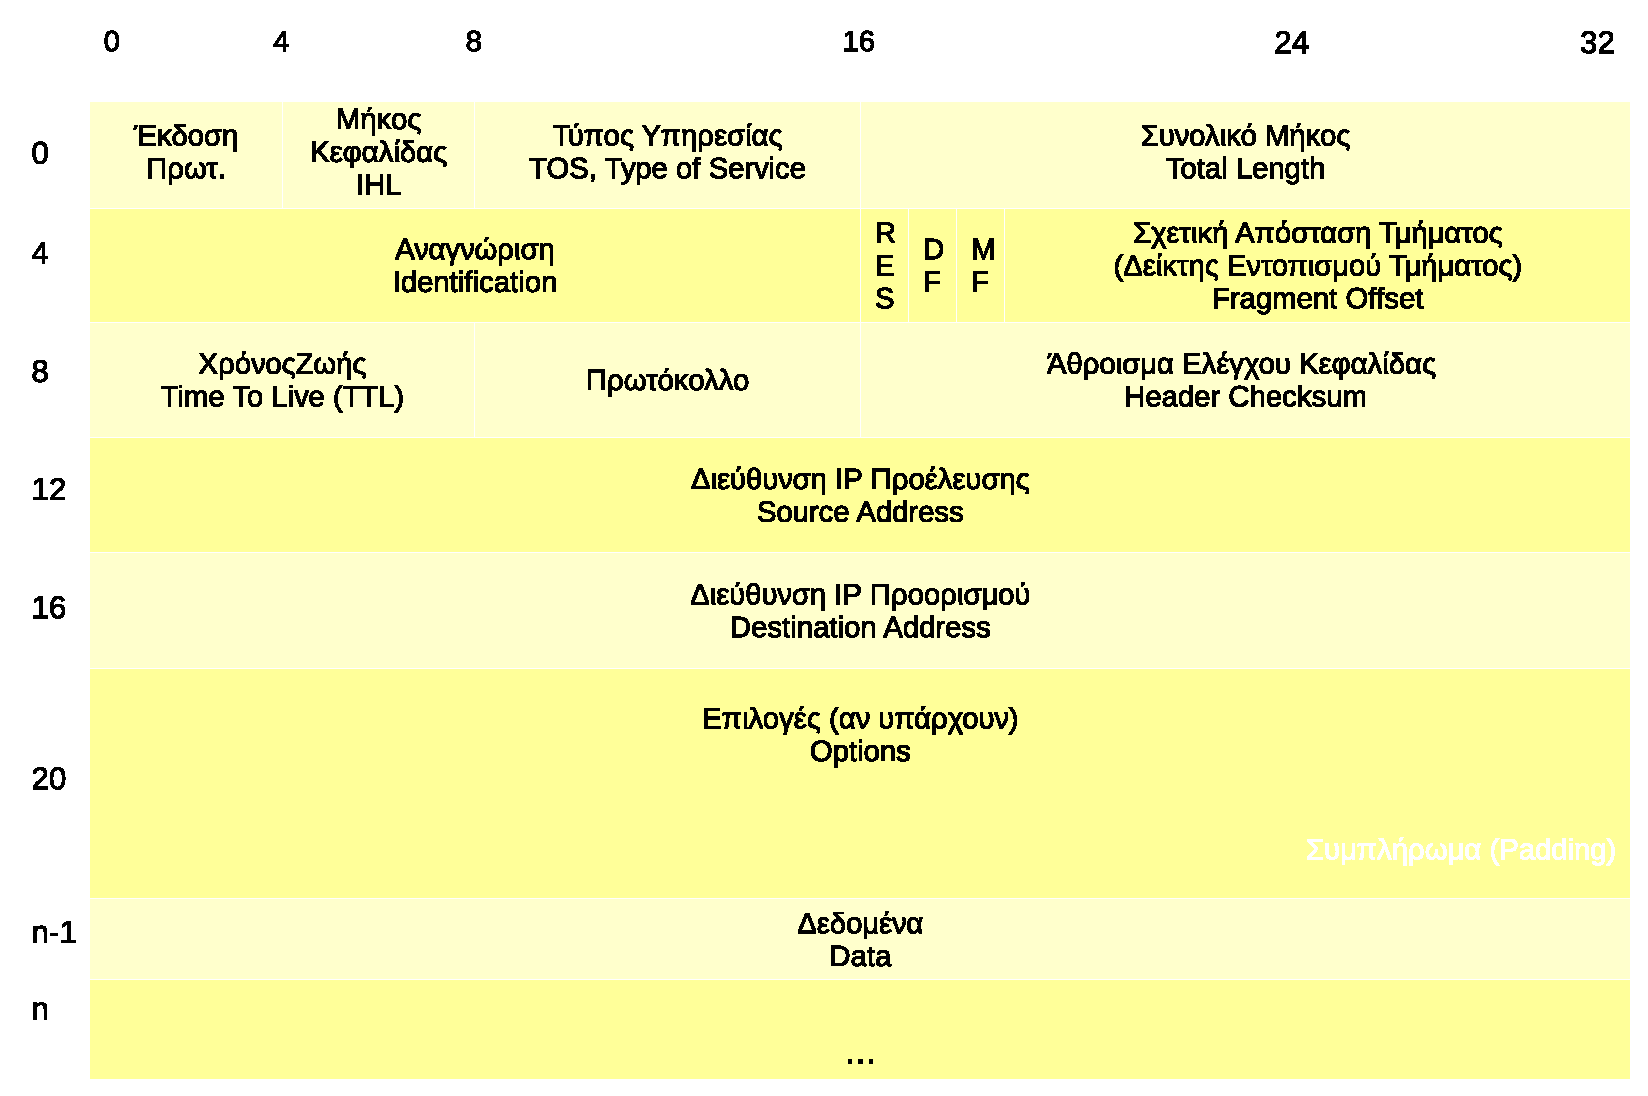
\includegraphics[width=0.95\textwidth]{images/chapter3/3-5}
  \caption {\textsl{Δομή Αυτοδύναμου Πακέτου IP}}
  \label{3-5}
\end{figure}

\begin{itemize}
\item \textbf{Έκδοση Πρωτοκόλλου:} Το πεδίο αυτό έχει μέγεθος 4 bit και δηλώνει την έκδοση του πρωτοκόλλου IP που χρησιμοποιείται. Έχει τις τιμές 4 για IPv4 και 6 για IPv6. Αν χρησιμοποιείται IPv6, η επικεφαλίδα έχει ελάχιστο μήκος 40 bytes.
\item \textbf{Μήκος Επικεφαλίδας:} Το πεδίο αυτό είναι μήκους 4 bit και εκφράζει το μήκος της επικεφαλίδας σε λέξεις των 32bit. Έτσι αν έχει τιμή 5, η επικεφαλίδα είναι 32Χ5=160 bit και άρα 160/8=20 bytes. Μπορείτε επίσης να πολλαπλασιάσετε την τιμή του πεδίου αυτού με το 4 για να βρείτε απευθείας το μήκος της επικεφαλίδας σε bytes.

\begin{inthebox}
\textbf{Προσέξτε} ότι στις ασκήσεις άλλες φορές δίνεται το μήκος της επικεφαλίδας σε bytes (π.χ. 20 bytes) και άλλες \textbf{η τιμή του πεδίου ``μήκος επικεφαλίδας''} οπότε πρέπει να πολλαπλασιάσουμε με το 4 για να βρούμε τα bytes της επικεφαλίδας.\\
\end{inthebox}

Το ελάχιστο μήκος επικεφαλίδας είναι 5 λέξεις των 32 bit ή 20 bytes και το μέγιστο 15 λέξεις ή 60 bytes (4X15).
\item \textbf{Τύπος Υπηρεσίας:} Το πεδίο αυτό έχει μήκος 8 bit και περιγράφει τον επιθυμητό χειρισμό του πακέτου από κάθε κόμβο που θα περάσει. Μπορεί να δίνεται προτεραιότητα στην ταχύτητα, εάν δηλ. επιτρέπεται να καθυστερήσει ή όχι, στην αξιοπιστία ή στο ρυθμό διακίνησης (throughput). Με νεώτερη αναθεώρηση, το \href{https://tools.ietf.org/html/rfc2474}{RFC2474} αλλάζει τη σημασία του συγκεκριμένου πεδίου ώστε να υποστηρίζει ένα σύνολο διαφοροποιημένων υπηρεσιών που ονομάζει \emph{Differentiated Services Code Point - DSCP (6 bit)}. Τα υπόλοιπα 2 bit χαρακτηρίζονται από το \href{https://tools.ietf.org/html/rfc3168}{RFC3168}  ως ρητή ειδοποίηση συμφόρησης, \emph{Explicit Congestion Notification, ECN}. Οι αλλαγές αυτές έγιναν με σκοπό να υποστηρίξουν νέες υπηρεσίες με ιδιαίτερες απαιτήσεις όπως η μεταφορά φωνής μέσω VoIP. Για να είναι εφικτό αυτό, πρέπει οι υπηρεσίες να υποστηρίζονται και από το υπόλοιπο δίκτυο. 

\item \textbf{Συνολικό Μήκος:} Το πεδίο αυτό έχει μέγεθος 16 bits και δηλώνει το συνολικό μήκος (επικεφαλίδα και δεδομένα) του πακέτου σε bytes. Η ελάχιστη τιμή που μπορεί να πάρει είναι 20 (αντιπροσωπεύει ένα πακέτο με μόνο το βασικό, σταθερό τμήμα της επικεφαλίδας χωρίς καθόλου δεδομένα) και η μέγιστη 65535 (τιμή που αντιστοιχεί σε 16 άσους). Αυτό σημαίνει ότι το \emph{μέγιστο μέγεθος του αυτοδύναμου πακέτου IP} στο IPv4 είναι 65535 bytes (πρακτικά, 64 Kbyte).

\item \textbf{Αναγνώριση:} Καθώς το πακέτο IP κινείται προς τον προορισμό του, ενδέχεται να περάσει από αρκετά ενδιάμεσα δίκτυα.Το μέγιστο μήκος δεδομένων που μπορεί να μεταδοθεί σε ένα πλαίσιο από το επίπεδο ζεύξης δεδομένων ενός δικτύου, είναι γνωστό με την ονομασία \emph{MTU, Maximum Transfer Unit}. Έτσι, για παράδειγμα το Ethernet έχει MTU 1500 bytes (κάθε πλαίσιο Ethernet μπορεί να μεταδώσει μέχρι 1500 bytes δεδομένων). Διαφορετικοί τύποι δικτύων έχουν άλλο MTU. Ένα πακέτο IP ενδέχεται να έχει μέγεθος τέτοιο που να μην μπορεί να μεταδοθεί από ένα ενδιάμεσο δίκτυο χωρίς να διασπαστεί περισσότερο. 

Στην περίπτωση αυτή, αν το πακέτο επιτρέπεται να διασπαστεί, θα χωριστεί σε τμήματα που ονομάζονται \emph{fragments}. Η διαδικασία είναι γνωστή ως \emph{διάσπαση ή κατάτμηση (IP Fragmentation)}. Όταν τα τμήματα φτάσουν στο προορισμό τους θα πρέπει να επανασυνδεθούν για να σχηματίσουν ξανά το αρχικό πακέτο IP. Καθώς στον παραλήπτη μπορεί να φτάνουν τμήματα από πακέτα IP που προέρχονται από διαφορετικές επικοινωνίες, το πεδίο \emph{Αναγνώριση} περιέχει ένα αριθμό που χρησιμοποιείται για να αναγνωριστούν ποια τμήματα ανήκουν σε κάθε πακέτο: όλα τα τμήματα που προέρχονται από τη διάσπαση ενός συγκεκριμένου πακέτου έχουν τον ίδιο αριθμό αναγνώρισης στην επικεφαλίδα τους.

\item \textbf{Σχετική Θέση Τμήματος ή Δείκτης Εντοπισμού Τμήματος:} Και αυτό το πεδίο (όπως και η Αναγνώριση) χρησιμοποιείται στην περίπτωση που έχουμε διάσπαση. Χρησιμοποιείται για να μπουν ξανά τα fragments στη σωστή σειρά στον υπολογιστή προορισμού. Το πεδίο έχει μέγεθος 13 bits και ο αριθμός που περιέχει εκφράζει την απόσταση του τμήματος από το πρώτο σε οκτάδες (8x) byte. Η σχετική θέση τμήματος είναι πάντοτε μηδέν στο πρώτο τμήμα. Στα επόμενα τμήματα, την υπολογίζουμε διαιρώντας τα καθαρά δεδομένα (χωρίς επικεφαλίδα) που έχουν μεταδοθεί μέχρι εκείνη τη στιγμή  με το οκτώ.

Για παράδειγμα, αν διασπάσουμε ένα πακέτο συνολικού μήκους 1500 bytes σε δίκτυο με MTU 500 bytes:

\begin{itemize}
\item Τα δεδομένα του αρχικού πακέτου είναι 1500 bytes - 20 bytes επικεφαλίδα = 1480 bytes
\item Το πρώτο τμήμα θα έχει Σχετική Θέση Τμήματος μηδέν και συνολικό μήκος 500 bytes. Από αυτά, τα 20 είναι επικεφαλίδα. Συνολικά θα μεταδώσουμε 480 bytes καθαρών δεδομένων.
\item Το δεύτερο τμήμα θα έχει Σχετική Θέση Τμήματος 480/8 = 60 (τα δεδομένα που μεταδώσαμε στο πρώτο fragment δια οκτώ) και θα είναι επίσης 500 bytes συνολικό μήκος. Θα περιέχει επίσης 480 bytes δεδομένων.
\item Το τρίτο τμήμα θα έχει Σχετική Θέση Τμήματος 960/8 = 120 (ή 2Χ60) και συνολικό μήκος 500 bytes. Θα περιέχει 480 bytes δεδομένων.
\item Για το τέταρτο και τελευταίο τμήμα έχουν μείνει 40 bytes δεδομένων, αφού έχουμε ήδη μεταδώσει 3Χ480=1440 bytes. Το συνολικό μήκος είναι 60 bytes και η Σχετική Θέση Τμήματος είναι 1440/8=180 (ή 3Χ60).
\end{itemize}   

Το σχολικό βιβλίο γράφει τον παρακάτω τύπο για τον υπολογισμό της σχετικής θέσης τμήματος:

\begin{center}
Fragment\_offset = n * INT((MTU - IHL * 4) / 8)
\end{center}

όπου το n συμβολίζει τον αριθμό του fragment (μηδέν για το πρώτο fragment) και το IHL το πεδίο ``μήκος επικεφαλίδας'' (με τιμή 5 για επικεφαλίδα 20 bytes). Πρακτικά, ο τύπος σημαίνει τα παρακάτω:

\begin{itemize}
\item Το πρώτο fragment έχει σχετική θέση τμήματος μηδέν (για n=0).
\item Για το δεύτερο fragment (n=1), η σχετική θέση τμήματος είναι τα καθαρά δεδομένα (χωρίς επικεφαλίδα) που μεταδώσαμε στο πρώτο fragment δια οκτώ.
\item Για τα επόμενα fragment, η σχετική θέση τμήματος είναι πολλαπλάσιο αυτής που υπολογίσαμε στο δεύτερο τμήμα (Για n>=2).
\item Αν στη σχετική θέση τμήματος δεν προκύπτει ακέραια τιμή, αποκόπτουμε τα δεκαδικά. Σε αυτή την περίπτωση όμως \textbf{θα πρέπει να υπολογίσουμε ξανά τα δεδομένα που μεταδόθηκαν, καθώς δεν είναι αυτά που υποθέσαμε αρχικά}. Θα δούμε σχετικό παράδειγμα στο τέλος της ενότητας.
\end{itemize}

\emph{Δεν χρειάζεται στην πραγματικότητα να μάθετε ή να αποστηθίσετε τον τύπο!}

\item \textbf{Το πεδίο DF:} Το πεδίο αυτό έχει μέγεθος 1 bit και είναι στην πραγματικότητα μια σημαία που δείχνει αν το πακέτο επιτρέπεται ή όχι να διασπαστεί \emph{(DF: Don't Fragment, Απαγόρευση Διάσπασης)}. Αν για κάποιο λόγο το αυτοδύναμο πακέτο δεν πρέπει να διασπαστεί, το πεδίο αυτό θα έχει τιμή 1.  Έτσι κατά τη δρομολόγηση του πακέτου θα επιλεχθεί διαδρομή τέτοια ώστε να μη χρειάζεται διάσπαση, ή, αν αυτό είναι αδύνατο, το πακέτο θα απορριφθεί (και ενδεχομένως να ειδοποιηθεί ο αποστολέας για αυτό το γεγονός). Στην έκδοση IPv6 η διάσπαση του πακέτου διενεργείται μόνο από τον υπολογιστή προέλευσης με βάση το μικρότερο MTU της διαδρομής (Path MTU, PMTU) και όχι από τους ενδιάμεσους δρομολογητές. 
 
\item \textbf{Το πεδίο MF:} Όταν ένα αυτοδύναμο πακέτο διασπαστεί σε τμήματα, αυτά φτάνουν με τυχαία σειρά στον παραλήπτη. Είναι πολύ εύκολο για τον παραλήπτη να βρει ποιο είναι το πρώτο fragment (είναι αυτό που έχει σχετική θέση τμήματος μηδέν). Από τη σχετική θέση τμήματος μπορούν επίσης να μπουν όλα τα επόμενα τμήματα στη σωστή σειρά αλλά δεν μπορούμε να γνωρίζουμε ποιο είναι το τελευταίο. Για αυτό το σκοπό χρησιμοποιείται η σημαία MF \emph{(More Fragments, Περισσότερα Τμήματα)}. Σε όλα τα τμήματα έχει τιμή 1, εκτός από το τελευταίο που έχει τιμή μηδέν, σηματοδοτώντας έτσι το τέλος των τμημάτων του συγκεκριμένου αυτοδύναμου πακέτου.

\item \textbf{Το πεδίο Χρόνος ζωής (TTL, Time To Live):} Το πεδίο αυτό έχει μήκος 8 bit. Ξεκινά από τον αποστολέα με μια αρχική τιμή (συνήθως 64) και μειώνεται κατά 1 σε κάθε δρομολογητή από τον οποίο διέρχεται το πακέτο. Όταν η τιμή του πεδίου γίνει μηδέν, το πακέτο καταστρέφεται και επιστρέφεται στον αποστολέα διαγνωστικό μήνυμα σφάλματος υπέρβασης χρόνου ζωής (time exceeded). Κάθε φορά που το πακέτο διέρχεται από ένα δρομολογητή, λέμε ότι έχουμε μια \emph{αναπήδηση (hop)}. Το πεδίο αυτό μπορεί να χαρακτηριστεί ως ανάστροφος μετρητής αναπηδήσεων (αφού μειώνεται σε κάθε αναπήδηση). Λειτουργεί ως όριο απόρριψης ενός πακέτου όταν αυτό έχει καθυστερήσει, έχει χαθεί στη διαδρομή, έχει λάθος διεύθυνση παραλήπτη ή για κάποιο άλλο λόγο περιφέρεται άσκοπα στο δίκτυο χωρίς να μπορεί να παραδοθεί. Χωρίς αυτό το πεδίο, σύντομα το Internet θα πλημμύριζε από προβληματικά πακέτα που δεν θα μπορούσαν να παραδοθούν και θα σταματούσε να λειτουργεί!

Το πεδίο αυτό χρησιμοποιείται επίσης με έξυπνο τρόπο στην εντολή \textbf{traceroute ή tracert}. Πρόκειται για μια διαγνωστική εντολή που μας επιτρέπει να δούμε την διαδρομή που ακολουθούν τα πακέτα μέχρι ένα προορισμό. Ένα παράδειγμα εκτέλεσης της φαίνεται παρακάτω:

\fontsize{9}{10}
\begin{verbatim}
[09:15:17][sonic@pegasus:~]$ traceroute freebsdworld.gr
traceroute to freebsdworld.gr (193.183.99.68), 64 hops max, 40 byte packets
 1  router (192.168.0.250)  0.632 ms  0.879 ms  0.710 ms
 2  80.107.108.106 (80.107.108.106)  6.730 ms  8.669 ms  10.213 ms
 3  79.128.226.245 (79.128.226.245)  11.123 ms  11.170 ms
    79.128.227.213 (79.128.227.213)  11.505 ms
 4  62.75.3.157 (62.75.3.157)  12.009 ms
    kolasr02-hu-0-8-0-0.ath.OTEGlobe.gr (62.75.3.17)  11.596 ms
    kolasr02-hu-0-1-0-0.ath.OTEGlobe.gr (62.75.3.137)  11.286 ms
 5  62.75.4.162 (62.75.4.162)  58.291 ms  57.891 ms
    62.75.4.114 (62.75.4.114)  58.056 ms
 6  xe-7-1-1.edge5.London1.Level3.net (195.50.118.169)  58.150 ms  57.645 ms
    xe-7-3-0.edge5.London1.Level3.net (212.187.138.117)  57.233 ms
 7  ae-122-3508.bar2.Milan1.Level3.net (4.69.159.126)  77.716 ms  78.636 ms
    ae-120-3506.bar2.Milan1.Level3.net (4.69.159.118)  79.893 ms
 8  212.73.241.130 (212.73.241.130)  78.258 ms  78.423 ms  78.586 ms
 9  217.171.38.134 (217.171.38.134)  78.732 ms  78.130 ms  79.205 ms
10  zms.gudgenet.com (193.183.99.68)  79.799 ms  79.910 ms  79.773 ms
\end{verbatim}
\normalsize

Η εντολή δουλεύει ως εξής: Αρχικά στέλνει ένα πακέτο προς τον προορισμό που έχουμε επιλέξει με TTL 1. Το πακέτο αυτό καταστρέφεται στον πρώτο δρομολογητή ο οποίος μας επιστρέφει διαγνωστικές πληροφορίες που εμφανίζονται από την traceroute. Έπειτα στέλνεται άλλο πακέτο με TTL 2 το οποίο καταστρέφεται στο δεύτερο δρομολογητή κ.ο.κ. Αυξάνοντας συνέχεια το TTL μπορούμε να ανιχνεύσουμε όλη τη διαδρομή που ακολουθεί το πακέτο μέχρι τον προορισμό.

\item \textbf{Το πεδίο Πρωτόκολλο:} Το πεδίο αυτό έχει μήκος 8 bit. Περιέχει μια αριθμητική τιμή που δηλώνει από ποιο πρωτόκολλο του αμέσως ανώτερου επιπέδου (μεταφοράς) προέρχονται τα δεδομένα που μεταφέρει το συγκεκριμένο IP πακέτο. Έτσι, πληροφορείται το πρωτόκολλο IP στον παραλήπτη προκειμένου να παραδώσει τα δεδομένα στο αντίστοιχο πρωτόκολλο του επιπέδου μεταφοράς. Για παράδειγμα, αν η τιμή είναι 6 τα δεδομένα προέρχονται από το TCP, ενώ αν είναι 17 από το UDP. Καθώς φαντάζεστε υπάρχουν πολλά περισσότερα πρωτόκολλα στο επίπεδο μεταφοράς εκτός από τα δύο βασικά (TCP, UDP). Μπορείτε να δείτε μια λίστα των πιθανών τιμών και αντίστοιχων πρωτοκόλλων για αυτό το πεδίο στο \href{https://en.wikipedia.org/wiki/List_of_IP_protocol_numbers}{σχετικό λήμμα της Wikipedia}. Ακόμα μπορείτε να δείτε τα περιεχόμενα του αρχείου /etc/protocols σε οποιοδήποτε υπολογιστή UNIX/Linux ή το αρχείο C:\textbackslash{}Windows\textbackslash{}System32\textbackslash{}drivers\textbackslash{}etc\textbackslash{}protocols σε υπολογιστή Windows.

\item \textbf{Το πεδίο Άθροισμα Ελέγχου Επικεφαλίδας (Header Checksum):} Πρόκειται για ένα πεδίο μήκους 16 bit. Το πεδίο διασφαλίζει την ακεραιότητα δεδομένων της επικεφαλίδας, αποθηκεύοντας ένα άθροισμα ελέγχου που προκύπτει από όλα τα υπόλοιπα πεδία της (το ίδιο το πεδίο δεν συμμετέχει στο άθροισμα, θεωρώντας ότι περιέχει τιμή μηδέν). Το άθροισμα ελέγχου αναφέρεται μόνο στην επικεφαλίδα και όχι στα δεδομένα. Καθώς το πακέτο περνάει από διάφορους δρομολογητές, κάποια πεδία της επικεφαλίδας αλλάζουν, έτσι θεωρείται αναγκαία η ύπαρξη πεδίου ελέγχου για να αποφευχθούν λάθη.  

\item \textbf{Το πεδίο Επιλογές (Options):} Είναι προαιρετικό και όταν χρησιμοποιείται, προφανώς η επικεφαλίδα μας είναι μεγαλύτερη από τη βασική των 20 bytes. Χρησιμοποιείται για ειδικές λειτουργίες, όχι όμως συχνά. Αν χρειάζεται, μαζί με τις Επιλογές, χρησιμοποιείται και το πεδίο \textbf{Συμπλήρωμα (padding)} το οποίο συμπληρώνει το πεδίο με μηδενικά ώστε η επικεφαλίδα να είναι πάντοτε ακέραιο πολλαπλάσιο των 32 bit.
\end{itemize} 

\subsection*{Παράδειγμα Κατάτμησης Αυτοδύναμου Πακέτου IP}

Έστω ότι έχουμε ένα αυτοδύναμο πακέτο IP το οποίο προέρχεται από ένα δίκτυο Token Ring (δακτυλίου με κουπόνι πρόσβασης)  και πρόκειται να παραδοθεί σε ένα υπολογιστή προορισμού ο οποίος βρίσκεται σε δίκτυο Ethernet (σχήμα \ref{3-6}).Τα δύο αυτά δίκτυα ενώνονται μεταξύ τους με ένα δρομολογητή IP. Το δίκτυο δακτυλίου έχει MTU = 4482 bytes, δηλ. το πλαίσιο του (επίπεδο 2) μπορεί να μεταφέρει 4482 bytes δεδομένων, ενώ στο Ethernet γνωρίζουμε ότι το MTU = 1500 bytes. Είναι φανερό ότι ένα πακέτο IP του Token Ring δεν μπορεί να μεταδοθεί χωρίς να υποστεί κατάτμηση. Η δημιουργία των τμημάτων γίνεται στο δρομολογητή, εφόσον βέβαια το πεδίο DF έχει τιμή μηδέν. Θα περιγράψουμε εδώ τη διαδικασία διάσπασης.

\begin{figure}[!ht]
  \centering
  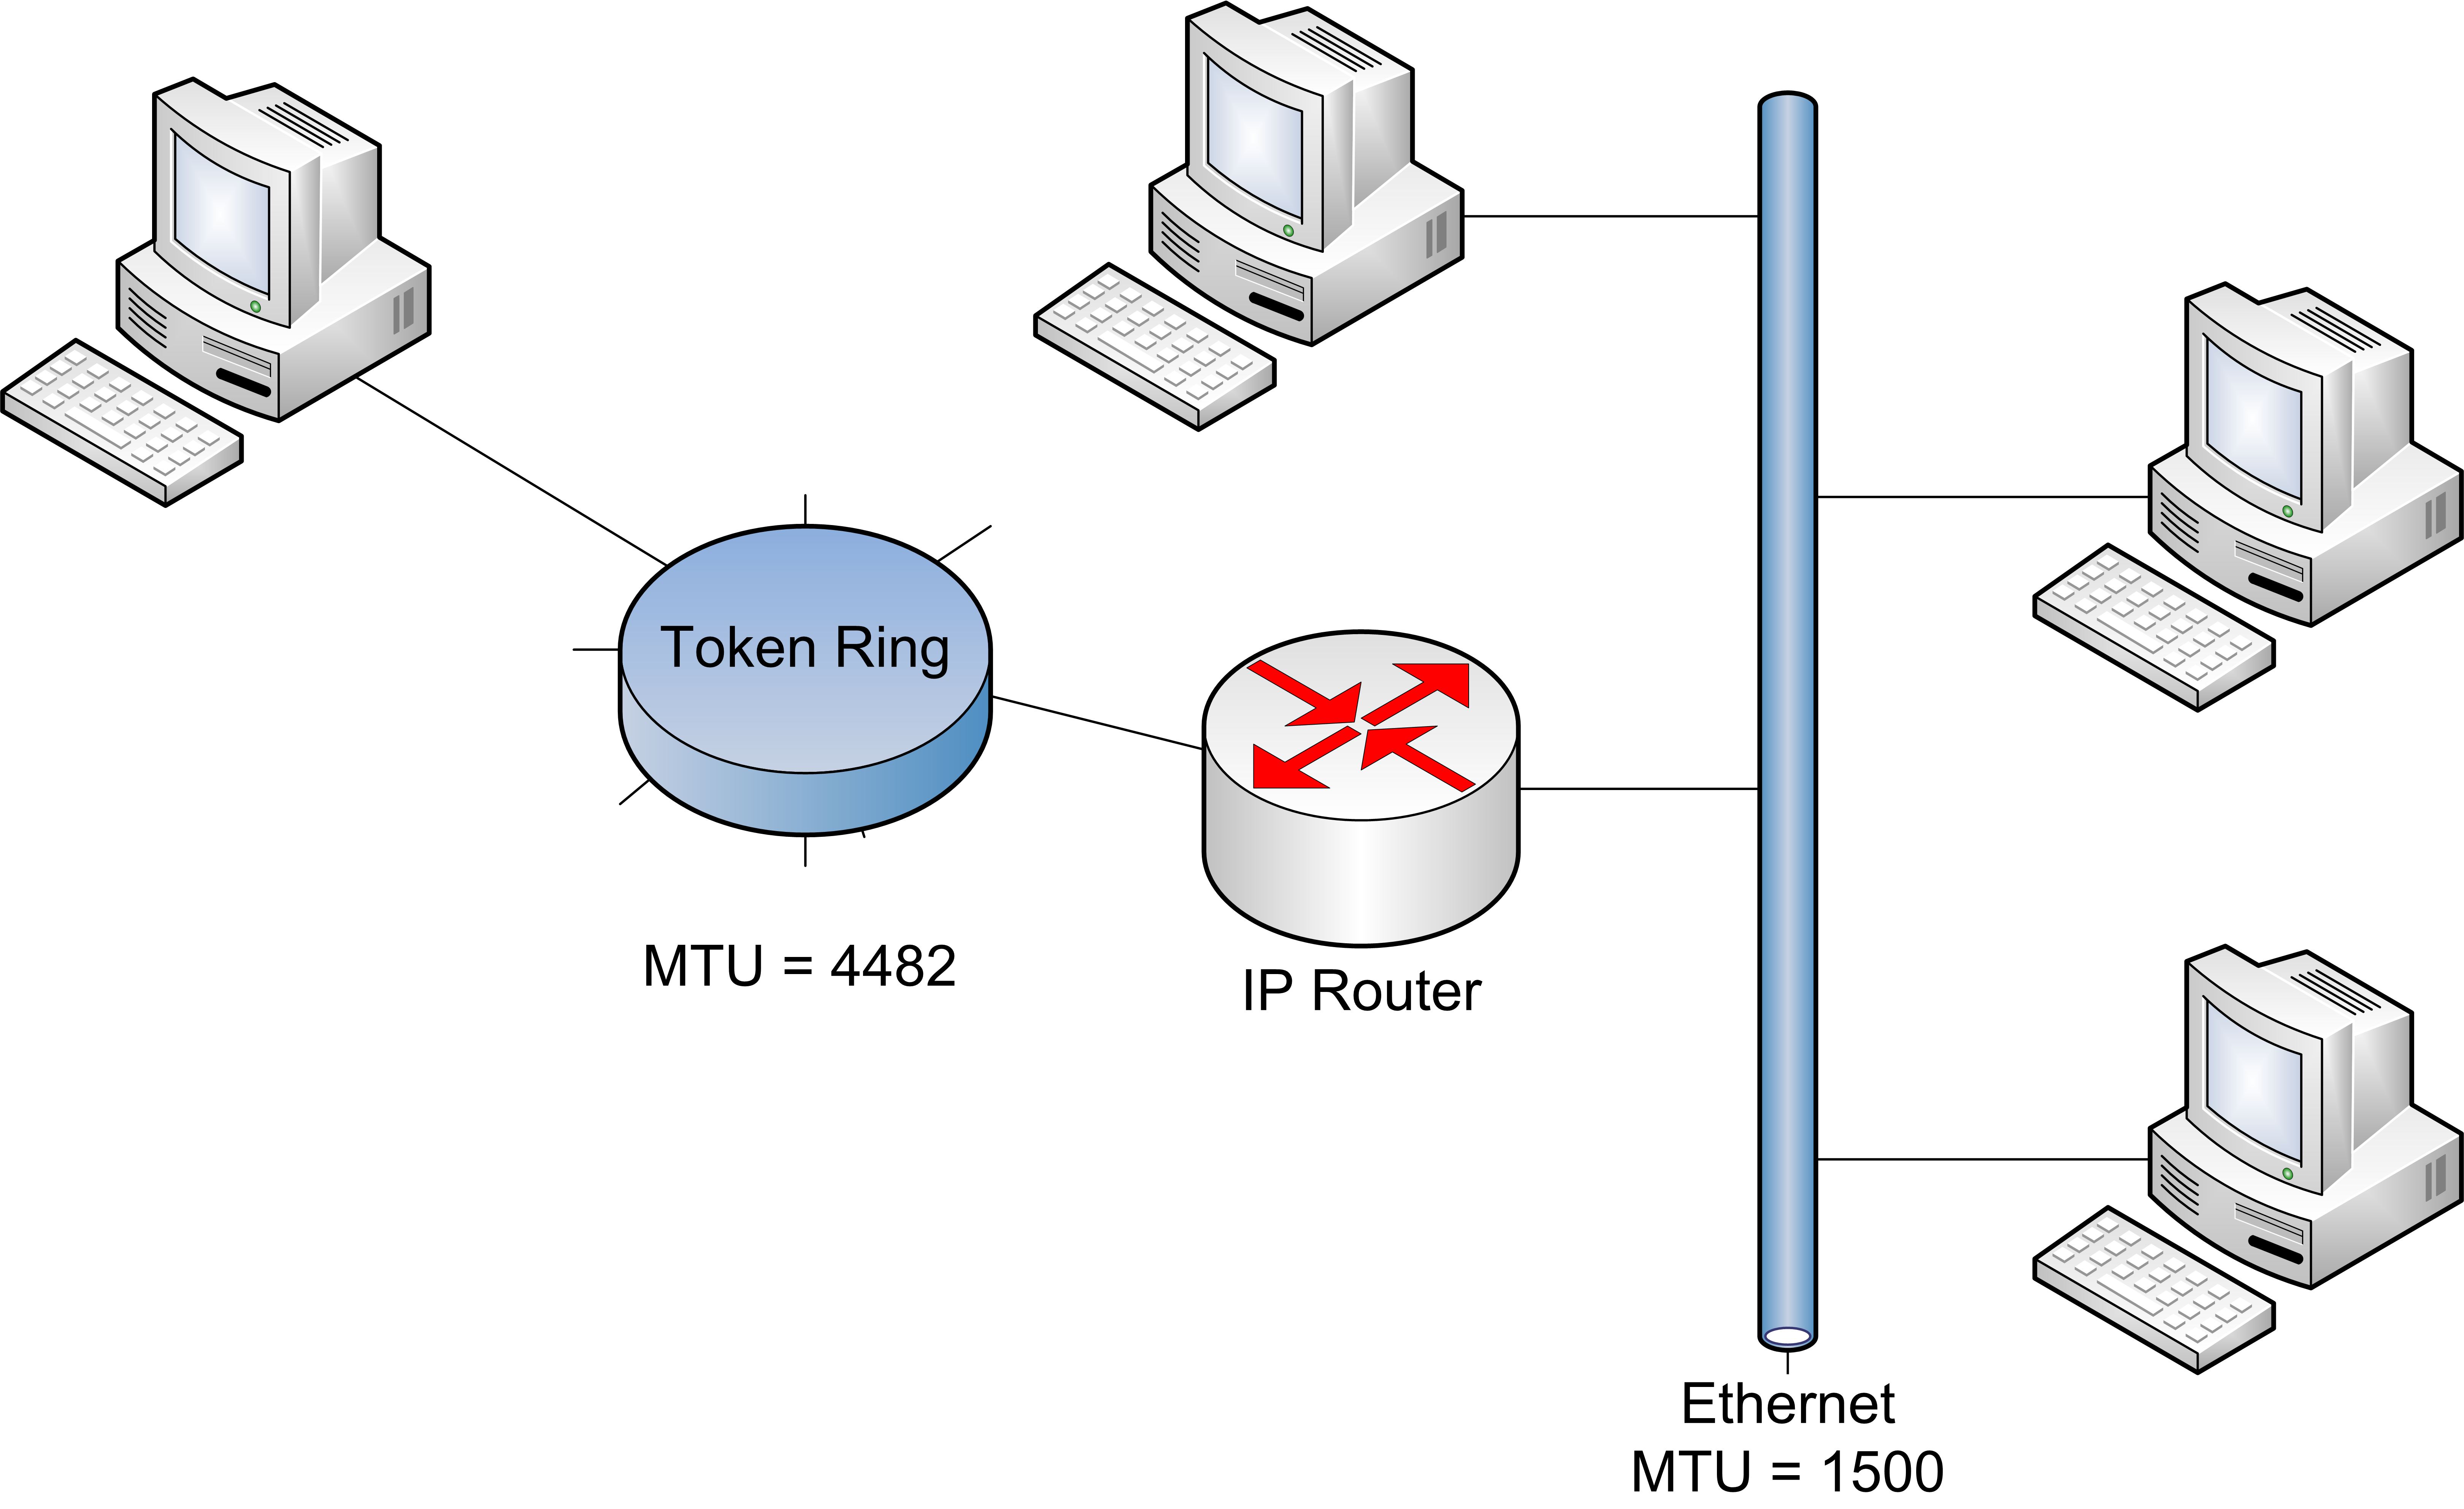
\includegraphics[width=0.95\textwidth]{images/chapter3/3-6}
  \caption {\textsl{Δίκτυα με Διαφορετικό MTU}}
  \label{3-6}
\end{figure}

\begin{itemize}
\item Το αρχικό πακέτο IP στο Token Ring έχει συνολικό μέγεθος 4482 bytes. Η επικεφαλίδα του είναι 20 bytes και περιέχει 4462 bytes δεδομένων.
\item Για να περάσει από το Ethernet θα πρέπει να διασπαστεί σε κομμάτια όχι μεγαλύτερα των 1500 bytes μαζί με την επικεφαλίδα. Κάθε τέτοιο κομμάτι θα περιέχει 1480 bytes δεδομένων.
\item Η Σχετική Θέση Τμήματος για το πρώτο τμήμα είναι μηδέν. Υπολογίζουμε τη Σχετική Θέση Τμήματος για το δεύτερο τμήμα διαιρώντας τα καθαρά δεδομένα του πρώτου με το οκτώ. 1480/8=185. Από τη διαίρεση προκύπτει ακέραιος αριθμός. \textbf{Επειδή δεν προκύπτουν δεκαδικά, τα τμήματα (εκτός από το τελευταίο) θα περιέχουν 1480 bytes δεδομένων όπως υποθέσαμε αρχικά.}
\end{itemize}

\begin{figure}[!ht]
  \centering
  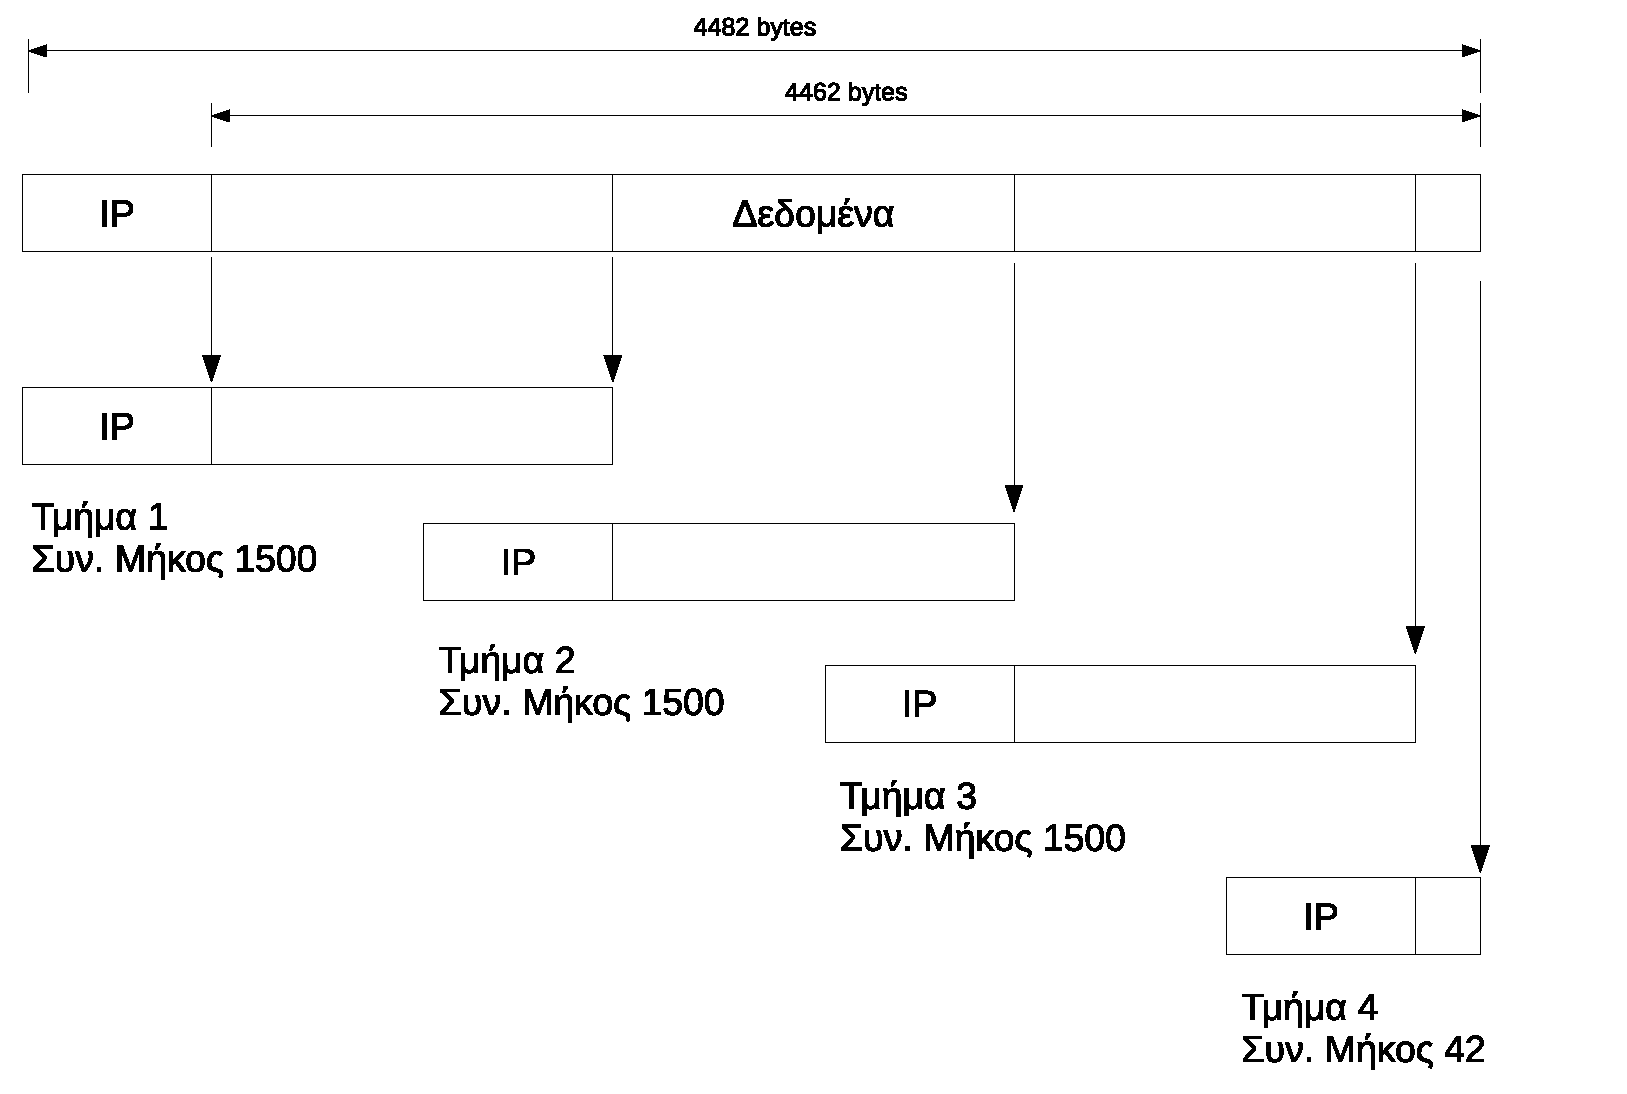
\includegraphics[width=0.95\textwidth]{images/chapter3/3-7}
  \caption {\textsl{Κατάτμηση Αυτοδύναμου Πακέτου IPv4}}
  \label{3-7}
\end{figure}

Πόσα τμήματα θα έχουμε; Στα πρώτα τρία τμήματα μεταδίδουμε 1480 bytes δεδομένων και απομένουν 22 bytes ακόμα για το τελευταίο, τέταρτο τμήμα. Το συνολικό μέγεθος για καθένα από τα τρία πρώτα τμήματα είναι 1500 bytes ενώ του τέταρτου 42 bytes. Η κατάτμηση φαίνεται στο σχήμα \ref{3-7}.
Το πεδίο ``Σχετική Θέση Τμήματος'' είναι μηδέν για το πρώτο τμήμα, 185 για το δεύτερο, 2Χ185=370 για το τρίτο, 3Χ185=555 για το τέταρτο τμήμα. Το πεδίο MF έχει τιμή 1 για όλα τα τμήματα εκτός του τελευταίου που έχει τιμή μηδέν.

\emph{Το σχολικό βιβλίο εφαρμόζει και πάλι τον τύπο, που δεν χρειάζεται να μάθετε!}

Όλα τα τμήματα του αρχικού πακέτου έχουν τον ίδιο αριθμό στο πεδίο ``Αναγνώριση''. Ο παραλήπτης χρησιμοποιεί τα πεδία MF και Σχετική Θέση Τμήματος για να βάλει τα τμήματα στη σωστή σειρά και να συναρμολογήσει ξανά το αρχικό αυτοδύναμο IP πακέτο. Τα τμήματα μπορεί να φτάσουν στον παραλήπτη με οποιαδήποτε σειρά. Παρακάτω δίνουμε τον πίνακα με τα πεδία για το κάθε τμήμα:

\begin{center}
\begin{tabular}{|c|c|c|c|c|}
\hline
& 1ο Τμήμα & 2ο Τμήμα & 3ο Τμήμα & 4ο Τμήμα \\
\hline
\multirow{2}{*}{} Πεδίο Μήκος Επικεφαλίδας & 5 & 5 & 5 & 5\\
(Λέξεις των 32 bit) & & & & \\
\hline
\multirow{2}{*}{} Συνολικό Μήκος & 1500 & 1500 & 1500 & 42 \\
(Bytes) & & & & \\
\hline
Μήκος Δεδομένων (Bytes) & 1480 & 1480 & 1480 & 22\\
\hline
Αναγνώριση & 0x2b41 & 0x2b41 & 0x2b41 & 0x2b41\\
\hline
DF (Σημαία) & 0 & 0 & 0 & 0\\
\hline
ΜF (Σημαία) & 1 & 1 & 1 & 0\\
\hline
\multirow{2}{*}{} Σχετική Θέση Τμήματος & 0 & 185 & 370 & 555\\
(Οκτάδες Byte) & & & & \\
\hline
\end{tabular}
\end{center}

\begin{figure}[!ht]
  \centering
  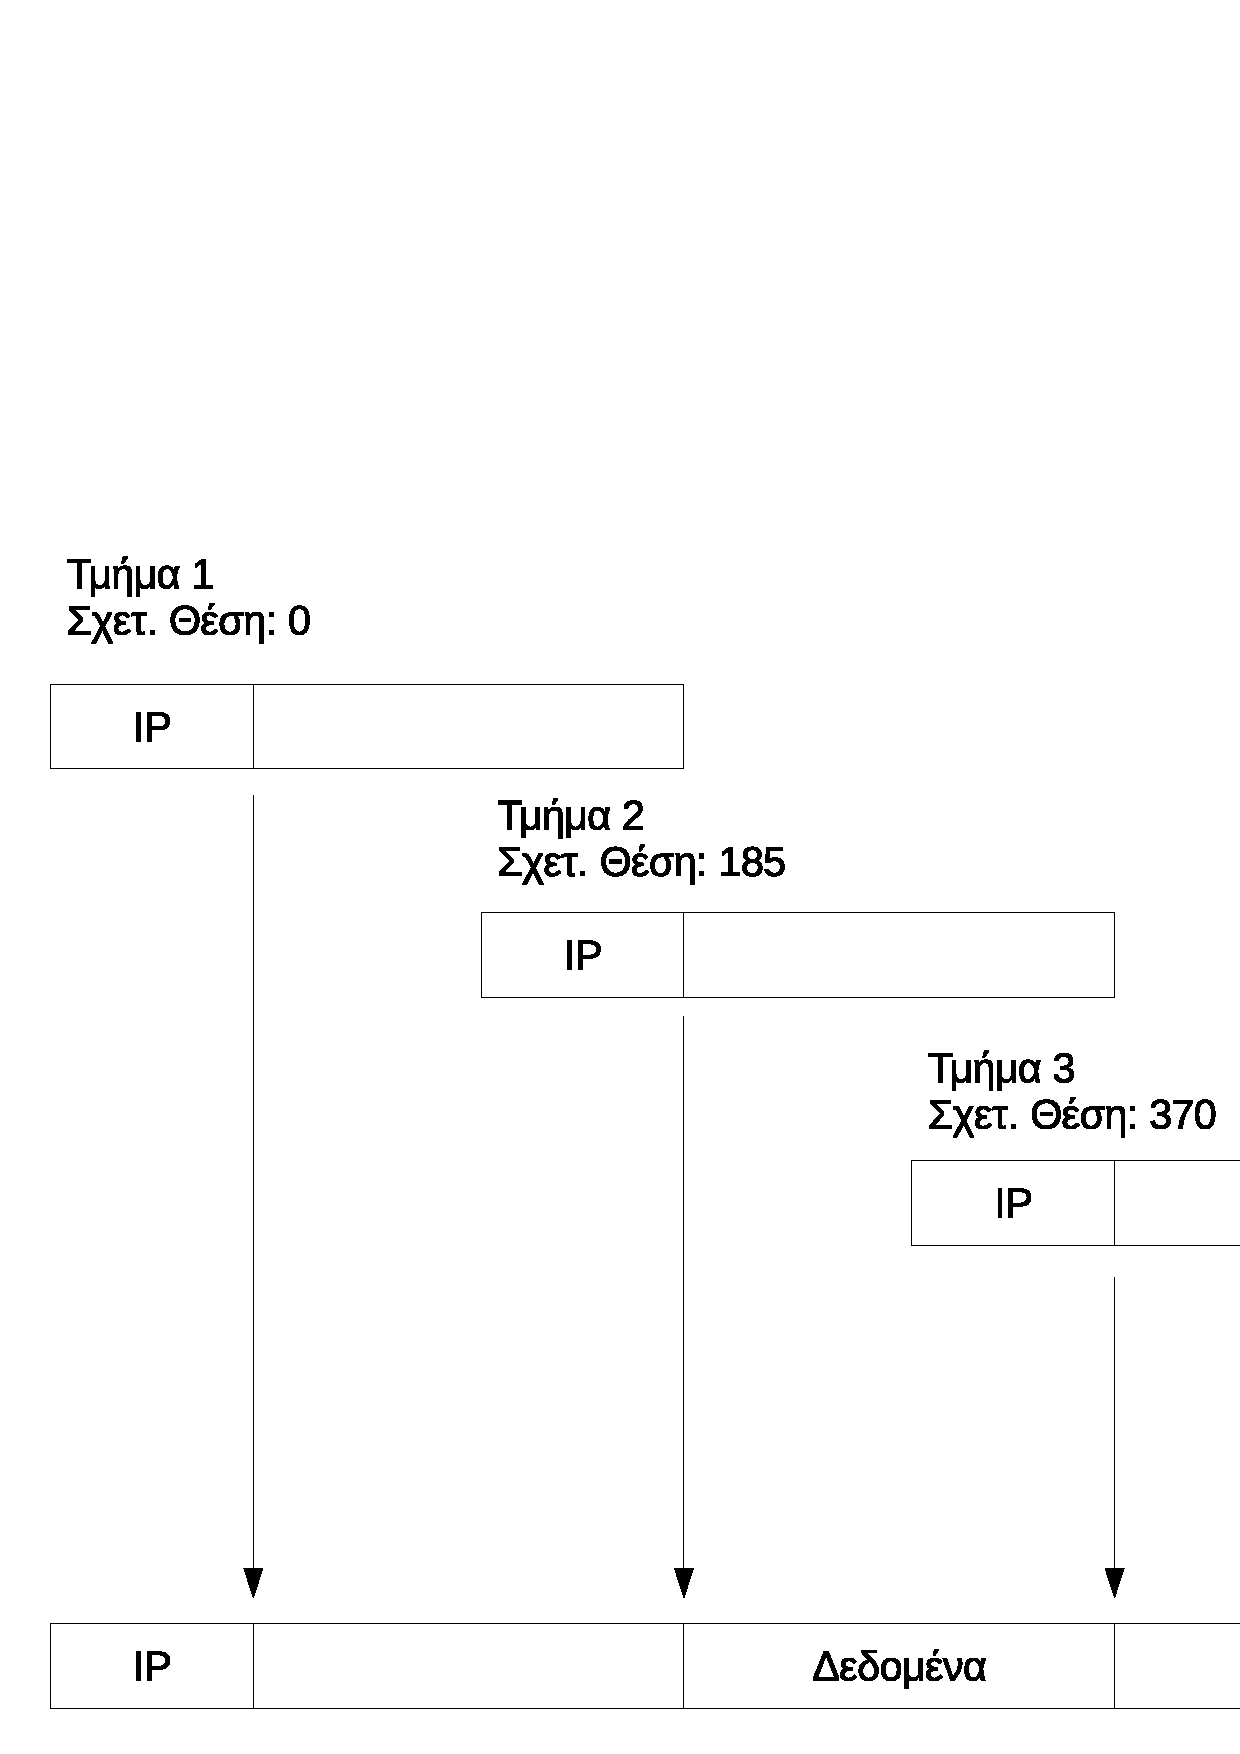
\includegraphics[width=0.95\textwidth]{images/chapter3/3-8}
  \caption {\textsl{Επανασύνθεση Πακέτου Από Τμήματα}}
  \label{3-8}
\end{figure}

\subsection*{Παράδειγμα Κατάτμησης Αυτοδύναμου Πακέτου IP \#2}

Στο παράδειγμα αυτό θα δούμε τι συμβαίνει αν κατά τον υπολογισμό της Σχετικής Θέσης Τμήματος προκύψει αριθμός με δεκαδικά ψηφία. 

Ένα αυτοδύναμο πακέτο με συνολικό μέγεθος 2400 bytes, DF=0 και Αναγνώριση 0x4a28 πρόκειται να διέλθει από δίκτυο το οποίο υποστηρίζει πακέτα συνολικού μεγέθους 1000 bytes (σχήμα \ref{3-9}).

\begin{figure}[!ht]
  \centering
  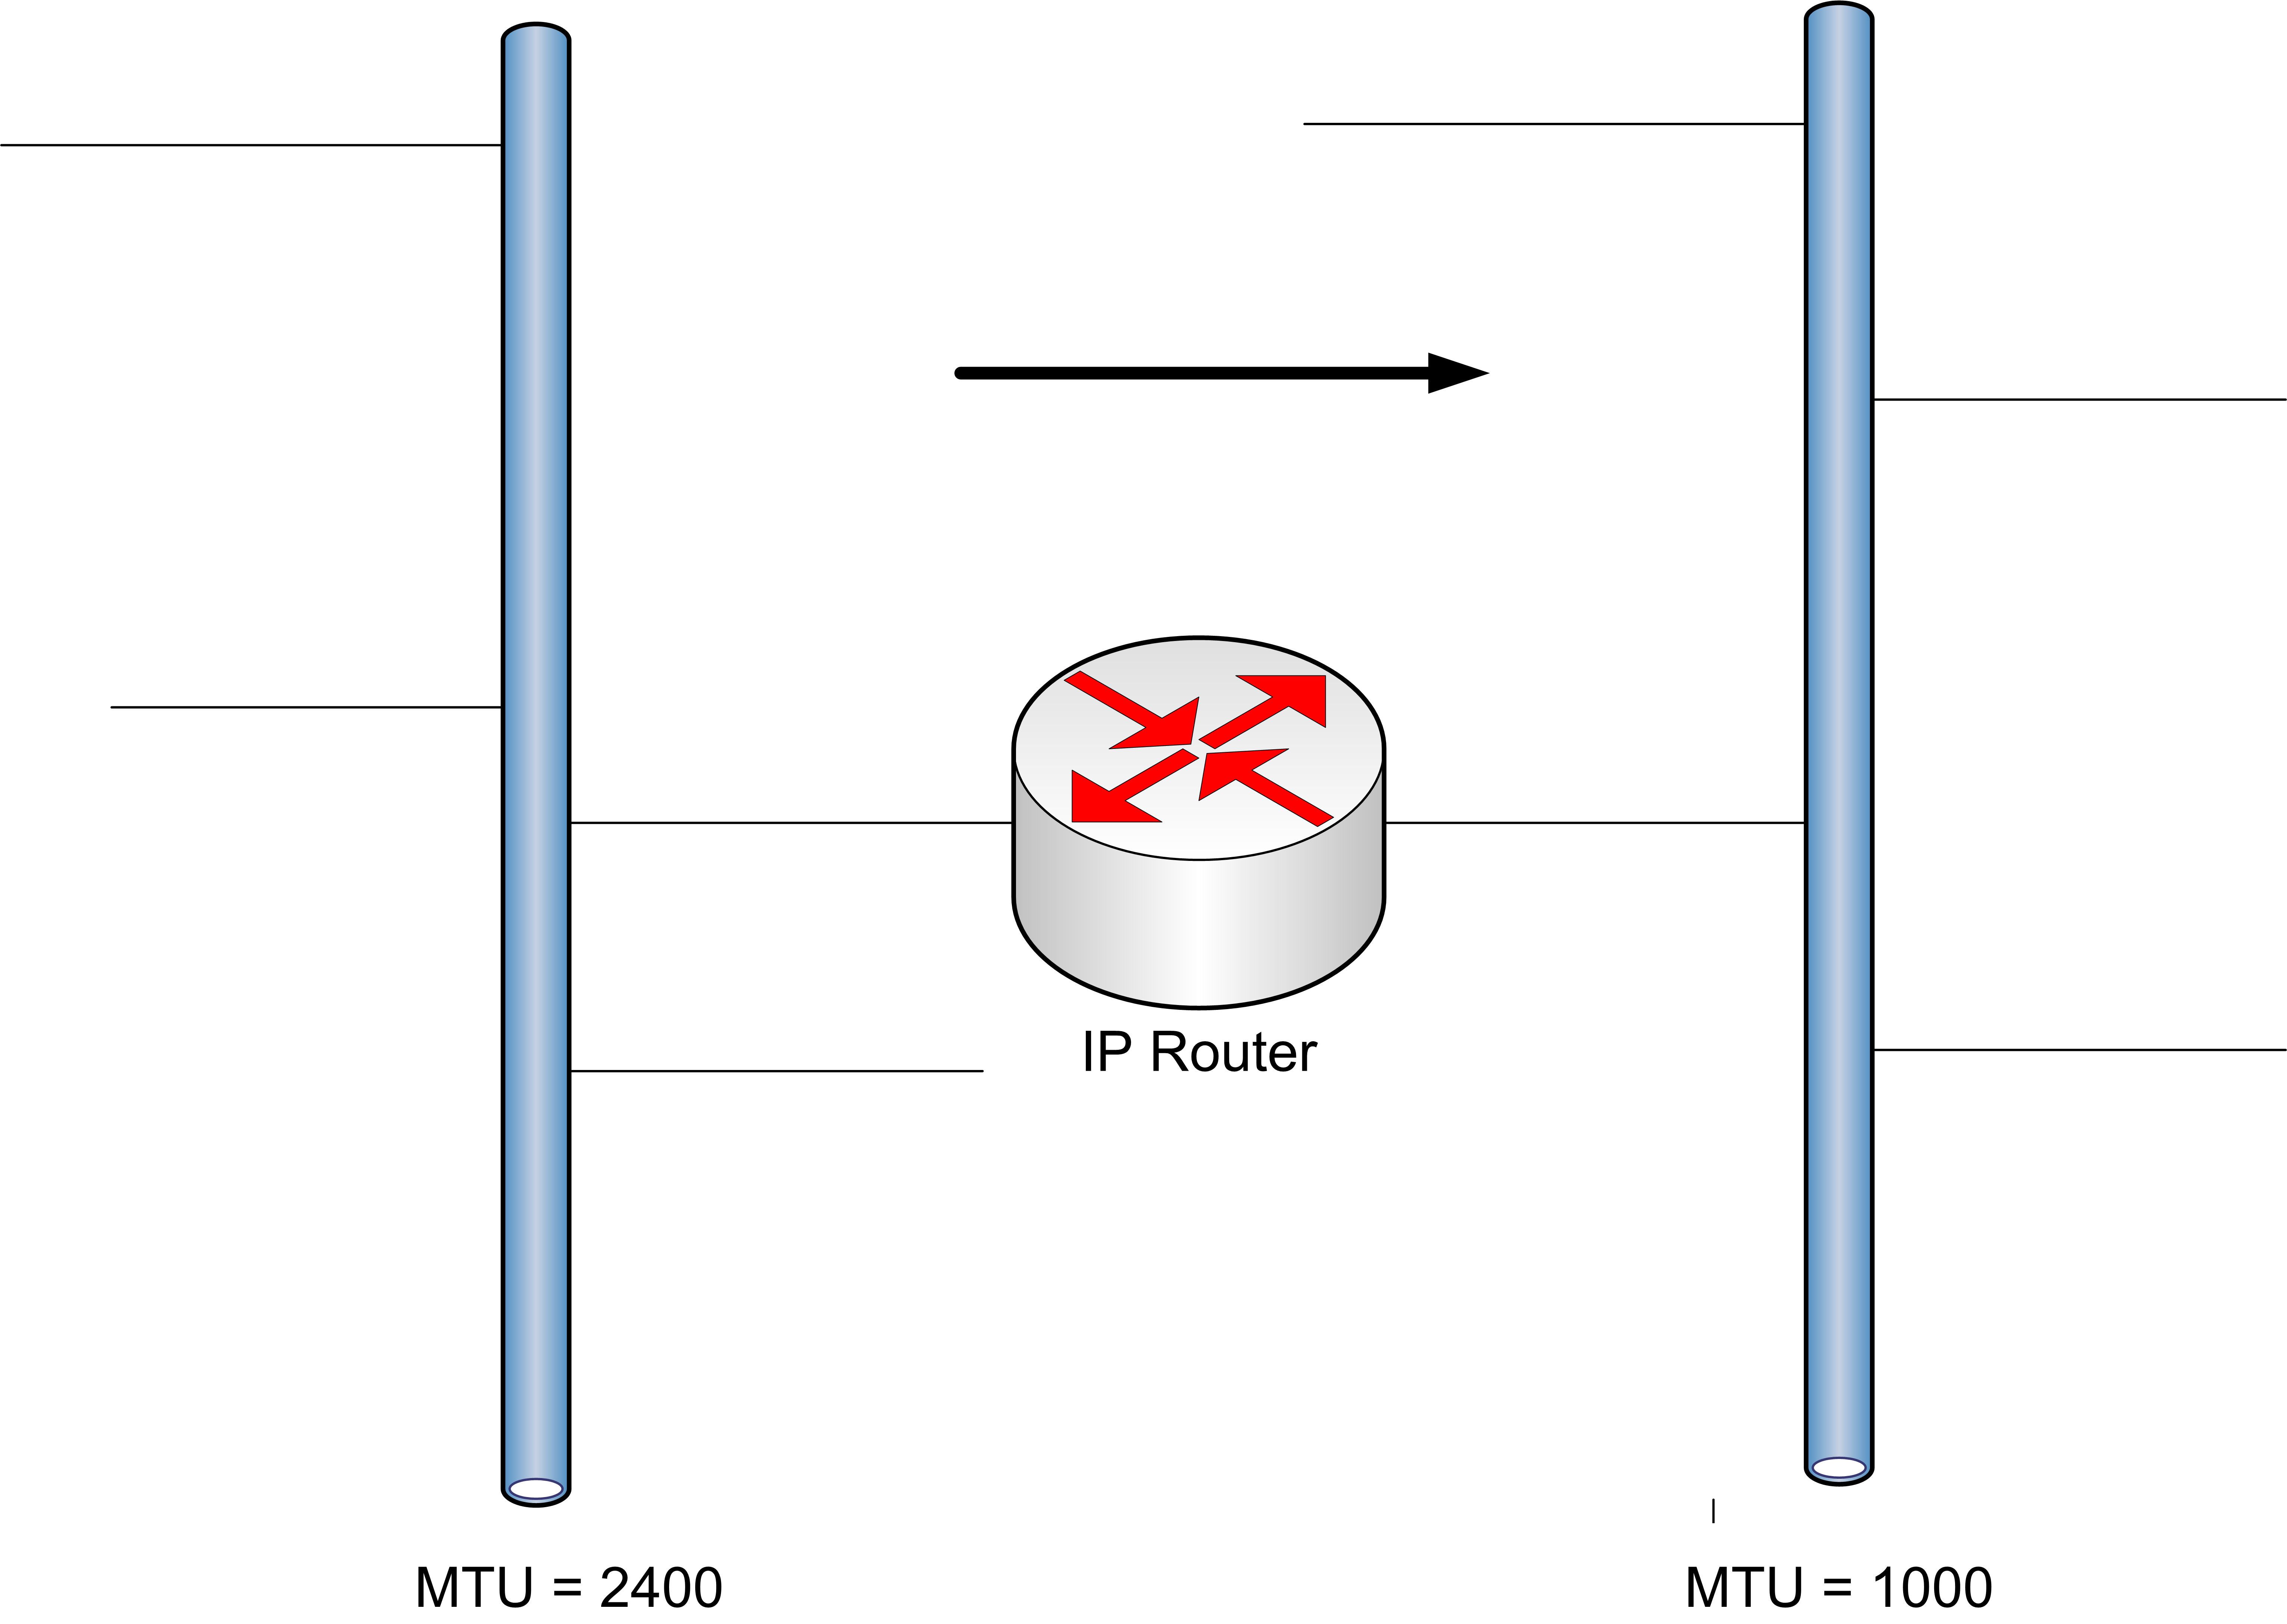
\includegraphics[width=0.60\textwidth]{images/chapter3/3-9}
  \caption {\textsl{Δίκτυα με Διαφορετικό MTU}}
  \label{3-9}
\end{figure} 

\begin{enumerate}
\item Θα γίνει κατάτμηση του πακέτου;
\item Αν ναι, δώστε τον πίνακα με τις τιμές των πεδίων Μήκος Επικεφαλίδας, Συνολικό Μήκος, Αναγνώριση, DF, MF και Σχετική Θέση Τμήματος (Offset).
\end{enumerate}

Στο πρώτο ερώτημα, η απάντηση είναι ναι, γιατί το πακέτο έχει DF=0 άρα η κατάτμηση επιτρέπεται.

Για το δεύτερο ερώτημα, ξέρουμε ότι το δίκτυο προορισμού υποστηρίζει πακέτα συνολικού μήκους 1000 bytes. Υποθέτουμε λοιπόν ότι το πακέτο μας θα γίνει τμήματα των 1000 bytes συνολικά. Το κάθε τμήμα όμως έχει 20 bytes επικεφαλίδα, άρα το μήκος δεδομένων του κάθε τμήματος θα είναι:

\begin{center}
1000 - 20 = 980 bytes
\end{center}

Η Σχετική Θέση Τμήματος για το πρώτο τμήμα είναι μηδέν. Για το δεύτερο τμήμα θα είναι:

\begin{center}
980 / 8 = 122.5
\end{center}

\textbf{Όμως η Σχετική Θέση Τμήματος δεν μπορεί να έχει δεκαδικά καθώς το μήκος δεδομένων του τμήματος διαιρείται πάντα ακριβώς με το οκτώ!} Αποκόπτοντας τα δεκαδικά, προκύπτει ότι η Σχετική Θέση Τμήματος για το δεύτερο τμήμα θα είναι 122.

Αυτό όμως σημαίνει ότι δεν μεταδώσαμε τελικά 980 bytes δεδομένων στο πρώτο τμήμα, \textbf{αλλά 122 Χ 8 = 976 bytes}. Όλα τα τμήματα μας θα έχουν αυτό το μήκος δεδομένων -- εκτός ενδεχομένως από το τελευταίο που θα είναι μικρότερο. Μπορούμε τώρα να φτιάξουμε τον πίνακα με τις τιμές των πεδίων του προβλήματος:

\begin{center}
\begin{tabular}{|c|c|c|c|}
\hline
& 1ο Τμήμα & 2ο Τμήμα & 3ο Τμήμα \\
\hline
\multirow{2}{*}{} Πεδίο Μήκος Επικεφαλίδας & 5 & 5 & 5\\
(Λέξεις των 32 bit) & & & \\
\hline
\multirow{2}{*}{} Συνολικό Μήκος & 996 & 996 & 448  \\
(Bytes) & & &  \\
\hline
Μήκος Δεδομένων (Bytes) & 976 & 976 & 428\\
\hline
Αναγνώριση & 0x2a28 & 0x2a28 & 0x2a28  \\
\hline
DF (Σημαία) & 0 & 0 & 0 \\
\hline
ΜF (Σημαία) & 1 & 1 & 0 \\
\hline
\multirow{2}{*}{} Σχετική Θέση Τμήματος & 0 & 122 & 244 \\
(Οκτάδες Byte) & & & \\
\hline
\end{tabular}
\end{center}

Για επιπλέον παραδείγματα, κατεβάστε επίσης τη \href{http://www.freebsdworld.gr/diktia/ipfragmentation.pdf}{Συνοπτική Μεθοδολογία Ασκήσεων IP Fragmentation}.